\section*{Exercice 189 -- SLCI -- Calculs}
\setcounter{exo}{0}
%CCS PSI 2015

On donne le schéma-blocs suivant.
\begin{center}
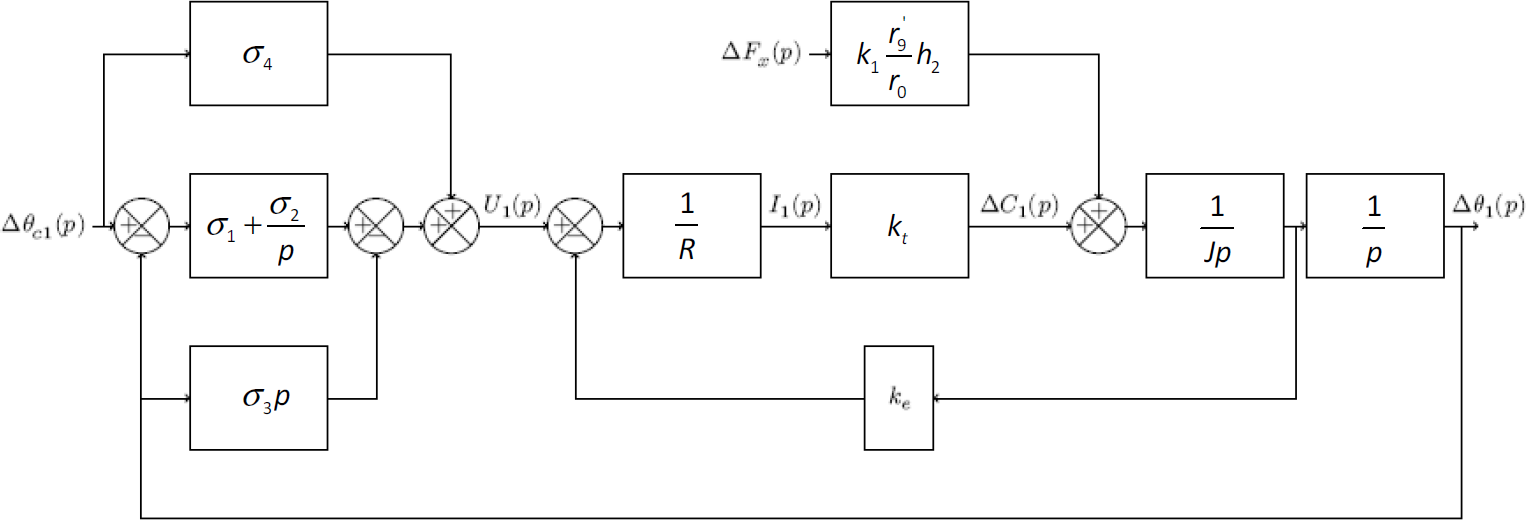
\includegraphics[width=\linewidth]{991_01}
\end{center}


\subparagraph{}
\textit{Exprimer la fonction de transfert en boucle fermée, sous forme canonique, notée $B_F(p)=\dfrac{\Delta \theta_1(p)}{\Delta \theta_{c1}(p)}$.}
\ifprof
\begin{corrige}
\end{corrige}
\else
\fi

